% !TEX root = main.tex
%=====================================================================
\chapter{Random processes}\label{chap:randomprocesses}

\newcommand{\Znn}{\mathbb{Z}_{\geq 0}}

%-------------------------------------------------
%\section{Random processes}\label{sec:rprocs}
Let $\Omega$ be the sample space of some random experiment and let $T\subseteq\R$ be a set of \emph{times}. The canonical examples are $T=\{0,1,2,\ldots\}$ which defines a discrete-time process, and $T=[0,\infty)$ which defines a continuous-time process.

\begin{definition}
A \emph{random process} on $\Omega$ is a collection of random variables $\{X_t:t\in T\}$, where each $X_t:\Omega\to\R$ is a random variable on $\Omega$.
\ben
\it If $T$ is countable, $\{X_t\}$ is called a \emph{discrete-time} random process.
\it If $T$ is uncountable, $\{X_t\}$ is called a \emph{continuous-time} random process. 
\een
\end{definition}

We can think of a random process $\{X_t\}$ as a mapping:
\[
\begin{array}{rccl}
\{X_t\}: 	& T\times\Omega		& \to		& \R \\
			& (t,\omega)		& \mapsto	& X_t(\omega).
\end{array}
\]

\begin{definition}
For a fixed outcome $\omega\in\Omega$, the associated realisation $\{X_t(\omega):t\in T\}$ of the random process $\{X_t:t\in T\}$ is called a \emph{trajectory} or \emph{sample path} of the process. 
\end{definition}

If $T$ is a finite set then $\{X_t\}$ is random vector which is defined by its joint CDF. If $T$ is an infinite set (either countable or uncountable) it is not easy to define a CDF to describe $\{X_t\}$. To do it, we have to deal with the joint distributions of $(X_{t_1},X_{t_2},\ldots,X_{t_n})$ for all $n\in\N$ and all choices of $t_1,t_2,\ldots,t_n\in T$. These are called the \emph{finite-dimensional distributions} of the random process.

%-----------------------------
\subsection{The canonical probability space}

Let $\Omega = [0,1]^{\N}$ be the set of infinite sequences of real numbers from the unit interval $[0,1]$, let $\mathbf{\omega}\in\Omega$ and write this as
\[
\mathbf{\omega} = (\omega_0,\omega_1,\omega_2,\ldots).
\]
The $n$th term of the sequence is extracted by the random variable
\[
\begin{array}{rccl}
	\gamma_n:	& \omega			& \to		& [0,1] \\
				& \mathbf{\omega}	& \mapsto	& \omega_n.
\end{array}
\]
We state the following theorem without proof.
\begin{theorem}
There exists a probability measure $\prob$ on $\Omega)$ such that the random variables $\gamma_0,\gamma_1,\ldots$ are independent and uniformly distributed on $[0,1]$.
\end{theorem}

We think of the single outcome $\mathbf{\omega} = (\omega_0,\omega_1,\omega_2,\ldots)$ as the source of all randomness in our experiment, and all other quantities are deterministic functions of this outcome (random variables).

%-----------------------------
\subsection{The Bernoulli process}\label{sec:bernoulliprocs}
\begin{definition}
A random process $\{X_n\}$ consisting of independent and identically distributed $\text{Bernoulli}(p)$ variables is called the $\text{Bernoulli}(p)$ process.
\end{definition}

In terms of the canonical probability space,
\[
X_n = \begin{cases}
	1	& \gamma_n\leq p, \\
	0	& \text{otherwise.}
\end{cases}
\]
Trajectories of the Bernoulli process are binary sequences (of infinite length).

\begin{example}
Let $\{X_n\}$ be a $\text{Bernoulli}(p)$ process. If $p>0$, show that a `success' is eventually observed with probability $1$.
\begin{solution}
\bit
\it $E 		= \{\omega\in\Omega:X_n(\omega)=1 \text{ for some } n\}$
\it $E_n 	= \{\omega\in\Omega:X_m(\omega)=1 \text{ for some } m\leq n\}$
\it $E_1\subset E_2\subset E_3\subset\ldots$ is an expanding sequence, with $E=\cup_{n=1}^{\infty} E_i$.
\it By continuity, 
\[
\prob(E) = \lim_{n\to\infty}\prob(E_n) = \lim_{n\to\infty}\big(1 - (1-p)^n\big) = 1.
\]
\eit
\end{solution}
\end{example}

% ex: hitting times
\begin{example} 
Suppose have observed the first $n$ terms of a $\text{Bernoulli}(p)$ process. Let $\tau$ be the time until we next observe a `success'. Show that $\tau\sim\text{Geometric}(p)$.
\begin{solution}
\[
\tau = \min\{m>0:X_{n+m}=1\}. 
\]
Because the $X_i$ are independent,
\begin{align*}
\prob(\tau > m | X_1,X_2,\ldots,X_n)
	& = \prob(X_{n+1}=0,X_{n+2}=0,\ldots,X_{n+m}=0 | X_1,X_2,\ldots,X_n) \\
	& = \prob(X_{n+1}=0)\prob(X_{n+2}=0)\cdots\prob(X_{n+m}=0) \\
	& = (1-p)^{m}
\end{align*}
so $\tau\sim\text{Geometric}(p)$ with $\prob(\tau=m)=(1-p)^{m-1}p$.
\end{solution}
\end{example}

% ex: memoryless
\begin{exercise}
Show that the geometric distribution has the so-called memoryless property: if $\tau\sim\text{Geometric}(p)$, then
\[
\prob(\tau > m+n|\tau > n) = \prob(\tau > m).
\]
\begin{answer}
\begin{align*}
\prob(\tau > m+n|\tau > n) 
	& = \prob(\tau>m+n,\tau>n)/\prob(\tau>n) \\
	& = \prob(\tau>m+n)/\prob(\tau>n) \\
	& = (1-p)^{m+n}/(1-p)^n \\
	& = (1-p)^m \\
	& = \prob(\tau > m).
\end{align*}
\end{answer}
\end{exercise}

%-------------------------------------------------
%\subsection{The Poisson process}\label{sec:poissonprocess}


%-------------------------------------------------
\section{Random walks}\label{sec:rwalks}

%intro
The \emph{simple random walk} is the simplest model of a \emph{diffusion process}. We consider a particle which inhabits the set of integer points $\Z$ and at each (discrete) time step the particle moves either one step to the right with probability $p$ or one step to the left with probability $q=1-p$. 
\bit
\it For fixed $\omega$ the random variable $X_n$ describes the trajectory of the particle over time.
\it For fixed $n$ the random variable $X_n$ describes the (spatial) distribution of the particle at time $n$.
\eit

\begin{definition}
A discrete random process $\{X_n\}$ is called a  \emph{simple random walk} with parameter $p\in(0,1)$ if
\ben
\it $X_{n+1}-X_n$ is independent of $X_0,X_1,\ldots,X_n$, 
\it $\prob(X_{n+1} = X_n + 1) = p$ and $\prob(X_{n+1} = X_n - 1) = q$ where $q=1-p$.
\een
If $p=1/2$ the random walk is called \emph{symmetric}.
\end{definition}


% link with canonical probability space
In terms of the random variables $\gamma_n$ defined on the canonical probability space let us define a new sequence of random variables,
\[
\xi_n = \begin{cases}
	\phantom{-}1	& \gamma_n\leq p, \\
	-1	& \text{otherwise.}
\end{cases}
\]
\begin{lemma}
The random process $\{X_n\}$ where $X_n = X_0 + \sum_{k=1}^n \xi_k$ is a simple random walk.
\begin{proof}
\ben
\it The $\xi_n$ are independent (they are transforms of the $\gamma_n$, which are independent), so the increment $X_{n+1}-X_n$ is independent of $\xi_1,\xi_2,\ldots,\xi_n$, and because $X_0,X_1,\ldots,X_n$ are just linear combinations of $\xi_1,\xi_2,\ldots,\xi_n$, it follows that $X_{n+1}-X_n$ is independent of $X_0,X_1,\ldots,X_n$.
\it Because $\gamma_{n+1}\sim\text{Uniform}[0,1]$,
\begin{align*}
\prob(X_{n+1} = X_n + 1) 
	& = \prob(\xi_{n+1} = 1) \prob(\gamma_{n+1}\leq p) = p.
\prob(X_{n+1} = X_n - 1) 
	& = \prob(\xi_{n+1} = -1) \prob(\gamma_{n+1} > p) = 1-p.
\end{align*}
\een
\end{proof}
\end{lemma}

%-----------------------------
\subsection{Properties}

\begin{definition}
A \emph{stationary} random process is one whose behaviour does not change when shifted in time and space.
\end{definition}

\begin{lemma}
The simple random walk satisfies
\[
\begin{array}{lcll}
\prob(X_n=x\,|\,X_0=a) 
	& = & \prob(X_n=x+b\,|\,X_0=a+b) 	&\qquad\text{(spatial homogeneity), and} \\
\prob(X_n=x\,|\,X_0=a) 
	& = & \prob(X_{m+n}=x\,|\,X_m=a) 	&\qquad\text{(temporal homgeneity)}
\end{array}
\]
and is therefore a stationary process.
\begin{proof}
\[
\begin{array}{lll}
\prob(X_n=x|X_0=a) 
	& = \prob\left(a+\sum_{k=1}^n \xi_k = x\right) \\
	& = \prob\left((a+b)\sum_{k=1}^n \xi_k = x+b\right) = \prob(X_n=x+b|X_0=a+b) \\
\prob(X_n=x|X_0=a) 
	& = \prob\left(a+\sum_{k=1}^n \xi_k = x\right) \\
	& = \prob\left(a+\sum_{k=m+1}^{m+n} \xi_k = x\right) = \prob(X_{m+n}=x|X_m=a).
\end{array}
\]
\end{proof}
\end{lemma}

%%-----------------------------
%\begin{theorem}
%Let $\{X_n\}$ be a simple random walk with parameter $p$, and suppose that $X_0=0$. Then $X_n$ is a discrete random variable, with
%\[
%\prob(X_n=\ell) = \binom{n}{\frac{n+\ell}{2}} p^{(n+\ell)/2}q^{(n-\ell)/2}
%\quad\text{for } \ell\in\{-n,-n+2,\ldots,-2,0,2,\ldots n-2, n\},
%\]
%where $q=1-p$, and zero otherwise.
%\begin{proof}
%
%\end{proof}
%\end{theorem}

%--------------------------------------------------------------------------
\subsection{Sample paths}
%--------------------------------------------------------------------------
The motion of a particle can be represented by the sequence $\{(n,X_n)\,:\,n=0,1,2,\ldots\}$., which is called the \emph{trajectory} or \emph{path} of the particle. By convention, sample paths are plotted with time on the horizontal axis, and displacement on the vertical axis.

Any event can be expressed in terms of an appropriate set of paths: the probability of the event is the probability that one of the associated paths is realized. The set of sample paths therefore serves as a \emph{sample space} for analysing the simple random walk.

Let $C_n$ be the set of all possible paths of length $n$,
\[
C_n = \big\{(x_0,x_1,\ldots,x_n)\in\Z^{n+1}: x_{k+1}-x_k = \pm 1\text{ for } k=0,1,2,\ldots,n-1\big\}.
\]

The probability that the first $n$ steps of the random walk follows any particular path $\mathbf{x}=(x_0,x_1,\ldots,x_n)$ is $p^cq^d$ where
\bit
\it $c$ is the number of positive steps (right/up), and
\it $d$ is the number of negative steps (left/down).
\eit

%-------------------------
\subsubsection{The distribution of the particle at time $n$}
We can compute the PMF of $X_n$ by examining the ensemble of all possible paths over the first $n$ steps. Let $C_n(a,b)$ be the set of paths from $(0,a)$ to $(n,b)$,
\[
C_n(a,b) = \big\{\mathbf{x}\in C_n: x_0=a, x_n=b\}.
\]

% lemma: PMF of $X_n$
\begin{lemma}
The number of possible paths from $(0,a)$ to $(n,b)$ is 
\[
|C_n(a,b)| = \binom{n}{\frac{1}{2}(n+b-a)}
\]
provided that $(n+b-a)/2$ belongs to the set $\{0,1,2\ldots,n\}$. 
\end{lemma}
If $X_0=0$, the condition says that the particle can occupy only odd-numbered sites after an odd number of steps, and only even-numbered sites after an even number of steps.)

\begin{proof}
Choose a path from $(0,a)$ to $(n,b)$. Let $u$ be the number of positive steps, and $d$ the number of negative steps.
\bit
\it $u+d=n$ is the total number of steps;
\it $u-d=b-a$ is the overall displacement to the right.
\eit
Solving for $c$ and $d$, we get $c=\frac{1}{2}(n+b-a)$ and $d=\frac{1}{2}(n-b+a)$. The number of paths from $(0,a)$ to $(n,b)$ is the number of ways of choosing exactly $u$ positive steps from the $n$ available steps, so
\[
|C_n(a,b)| = \binom{n}{u} = \binom{n}{\frac{1}{2}(n+b-a)}
\]
\end{proof}

% corollary: PMF of X_n
\begin{corollary}
%The probability that $X_n=b$ given that $X_0=a$ is 
\[
\prob(X_n=b|X_0=a) = \binom{n}{\frac{1}{2}(n+b-a)}p^{\frac{1}{2}(n+b-a)}q^{\frac{1}{2}(n-b+a)}
\]
\end{corollary}
\begin{proof}
Each path in $C_n(a,b)$ occurs with probability $p^{\frac{1}{2}(n+b-a)}q^{\frac{1}{2}(n-b+a)}$, so
\[
\prob(X_n=b|X_0=a) = \binom{n}{\frac{1}{2}(n+b-a)}p^{\frac{1}{2}(n+b-a)}q^{\frac{1}{2}(n-b+a)}
\]
\end{proof}

%--------------------------------------------------------------------------
\subsection{The Reflection Principle}
%--------------------------------------------------------------------------
Counting sample paths is made easier by using the \emph{reflection principle}.

\begin{figure}
\centering\resizebox{0.5\linewidth}{!}{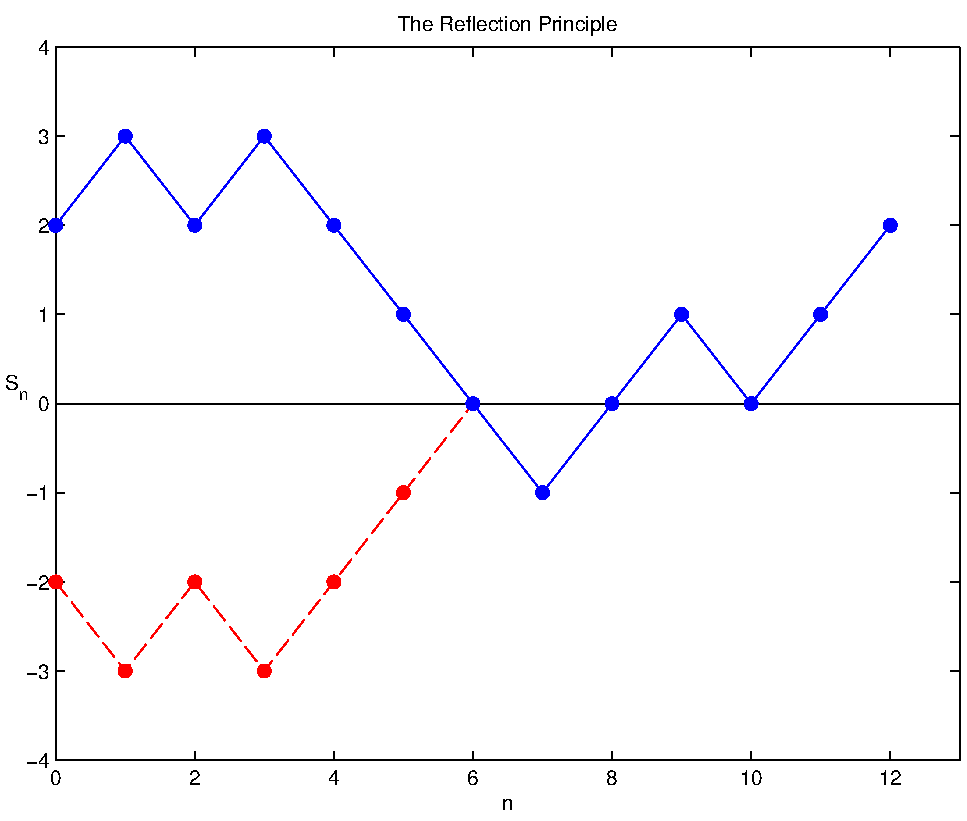
\includegraphics{reflection_principle}}
\caption{The Reflection Principle\label{reflection_principle}}
\end{figure}

%Let $a,b>0$ and define $C^{0}_n(a,b)$ to be the set of paths from $(0,a)$ to $(n,b)$ which contain a point of the form $(k,0)$, i.e.\ those trajectories which return to the (spatial) origin at some time step $k=0,1,2,\ldots,n$. We can use the reflection principle to show that the number of such paths is equal to the total number of paths from $(0,-a)$ to $(n,b)$.
%
%-------------------------
% theorem: reflection principle
\begin{theorem}
Let $a,b>0$, and let $C^{0}_n(a,b)$ be the set of paths from $(0,a)$ to $(n,b)$ which visit the (spatial) origin:% at some time step $k\in\{1,2,\ldots,n-1\}$,
\[
C^{0}_n(a,b) = \big\{\mathbf{x}\in C_n(a,b): x_k=a \text{ for some } k=1,2,\ldots,n-1\}.
\]
The number of such paths is equal to the total number of paths from $(0,-a)$ to $(n,b)$,
\[
|C^0_n(a,b)| = |C_n(-a,b)|.
\]
\end{theorem}
\begin{proof}
Each path from $(0,a)$ to $(n,b)$ intersects the horizontal axis at some earliest point $(k,0)$. If we reflect the segment of the path with $0\leq t\leq k$ in the horizontal axis, we obtain a path from $(0,a)$ to $(n,b)$ which intersects the horizontal axis. This operation puts the elements of $C^0_n(a,b)$ and $C_n(-a,b)$ in one-to-one correspondence, which proves the theorem.
\end{proof}

%For simplicity, we now focus our attention on simple random walks that start at the origin, i.e.\ those for which $X_0=0$.
%
%For $\ell > 0$, let $C^{*}_n(\ell)$ be the set of paths from $(0,0)$ to $(n,\ell)$ which do \emph{not} revisit the initial location $X_0=0$. 
%
%


%%--------------------------------------------------------------------------
%\subsubsection{The Ballot Theorem}
%
%For $b>a\geq 0$, let $C^{*}_n(a,b)$ to be the set of paths from $(0,a)$ to $(n,b)$ which do \emph{not} revisit the initial location $X_0=a$. 
%\[
%C^{*}_n(a,b) = \big\{\mathbf{x}\in C_n(a,b): x_k=0 \text{ for some } k=1,2,\ldots,n-1\}.
%\]

% ballot theorem
\begin{theorem}[The ballot theorem]
Let $b>a\geq 0$, and let $C^{*}_n(a,b)$ to be the set of paths from $(0,a)$ to $(n,b)$ which do \emph{not} revisit the initial location $X_0=a$, 
\[
C^{*}_n(a,b) = \big\{\mathbf{x}\in C_n(a,b): x_k=a \text{ for some } k=1,2,\ldots,n-1\}.
\]
The number of such paths is given by
\[
|C^{*}_n(a,b)| = \frac{b-a}{n} |C_n(a,b)|,
\]
where $C_n(a,b)$ is the set of all paths from $(0,a)$ to $(n,b)$.
\end{theorem}

%-------------------------
\begin{proof}
Without loss of generality, let $a=0$. The first step of all such paths must be to $(1,1)$, so by the reflection principle the number of such paths is
\begin{align*}
|C^{*}_n(0,b)|
	& = |C_{n-1}(1,b)| - |C^0_{n-1}(1,b)| \\
	& = |C_{n-1}(1,b)| - |C_{n-1}(-1,b)|
\end{align*}
The result then follows by the fact that the total number of paths $(0,0)$ to $(n,b)$ is equal to
\[
|C_n(0,b)| = \binom{n}{\frac{1}{2}(n+b)}
\]
and
\[
\begin{array}{lll}
|C_{n-1}(1,b)| 	& = \binom{n-1}{\frac{1}{2}(n+b)} 	& = \frac{n+b}{2n} |C_n(0,b)| \\
|C_{n-1}(-1,b)|	& = \binom{n-1}{\frac{1}{2}n+b-1}	& = \frac{n-b}{2n} |C_n(0,b)| \\
\end{array}
\]
\end{proof}

%-------------------------
% example
\begin{example}
In an election, candidate A scores $\alpha$ votes and candidate B scores $\beta$ votes, where $\alpha > \beta$. What is the probability that candidate $A$ was always ahead of candidate $B$ during the election? 
\begin{solution}
Assume that each possible combination of $\alpha$ votes for $A$ and $\beta$ votes for $B$ is equally likely.

\bigskip
After $n=\alpha+\beta$ steps, the required probability is the proportion of paths from $(0,0)$ to $(\alpha+\beta,\alpha-\beta)$ which do not re-visit the horizontal axis. By the ballot theorem, 
\[
\prob(\text{$A$ was always ahead of $B$}) = \frac{\alpha-\beta}{\alpha+\beta}.
\]
\end{solution}
\end{example}


%% thm: maximum
%\begin{theorem}
%Let $\{X_n\}$ be a symmetric simple random walk with $X_0=0$, and let $M_n=\max\{X_0,X_2,\ldots,X_n\}$. Then
%\[
%\prob(M_n\geq \ell)	= \prob(X_n=\ell) + \prob(X_n=\ell+1) 
%\]
%Note that only one of $\prob(X_n=\ell)$ and $\prob(X_n=\ell+1)$ is non-zero, the first if $n$ and $\ell$ are both odd or both even, and the second if one is odd and the other is even.
%\end{theorem}
%
%\begin{proof}
%Let $A_n(\ell)$ be the set of paths whose maximum is at least equal to $\ell$:
%\begin{align*}
%A_n(\ell) 
%	& = \{\mathbf{x}\in C_n: \max x_k \geq \ell, k=1,2,\ldots,n\} \\
%	& = \big\{\mathbf{x}\in C_n: x_k \geq \ell \text{ for at least one } k\in\{0,1,\ldots,n\}\big\}
%\end{align*}
%There are $2^n$ possible sample paths, all equally likely, so 
%\[
%\prob(M_n \geq \ell) = 2^{-n}|A_n(\ell)|.
%\]
%Let 
%\bit
%\it $A_n^{(1)}(\ell) = \big\{\mathbf{x}\in A_n(\ell): x_n > \ell\big\}$,
%\it $A_n^{(2)}(\ell) = \big\{\mathbf{x}\in A_n(\ell): x_n = \ell\big\}$,
%\it $A_n^{(3)}(\ell) = \big\{\mathbf{x}\in A_n(\ell): x_n < \ell\big\}$.
%\eit
%Then
%\[
%|A_n(\ell)| = |A_n^{(1)}(\ell)| + |A_n^{(2)}(\ell)| + |A_n^{(3)}(\ell)|
%\]
%
%By the reflection principle, the trajectories in $A_n^{(1)}(\ell)$ are in one-to-one correspondence with those in $A_n^{(3)}(\ell)$, so 
%\[
%|A_n(\ell)| = 2|A_n^{(1)}(\ell)| + |A_n^{(2)}(\ell)|
%\]
%
%Now, 
%\bit
%\it $A_n^{(1)}(\ell) = \cup_{k=\ell+1}^{\infty}\{\mathbf{x}: x_n=k\}$ and 
%\it $A_n^{(2)}(\ell) = \{\mathbf{x}: x_n=\ell\}.
%\eit
%
%There are $2^n$ sample paths, each equally likely, so
%\begin{align*}
%\prob(M_n\geq \ell)
%	& = 2\sum_{k=\ell+1}^{\infty}\prob(X_n=k) + \prob(X_n=\ell) \\
%	& = \sum_{k=\ell+1}^{\infty}\prob(X_n=k) + \sum_{k=\ell}^{\infty}\prob(X_n=\ell) \\
%\end{align*}
%
%Hence,
%\begin{align*}
%\prob(M_n = \ell) 
%	& = \prob(M_n\geq \ell) - \prob(M_n\geq \ell+1) \\
%	& = \prob(M_n\geq \ell) - \prob(M_n\geq \ell+1) \\
%	& = \left(\sum_{k=\ell+1}^{\infty}\prob(X_n=k) + \sum_{k=\ell}^{\infty}\prob(X_n=k)\right)
%			- \left(\sum_{k=\ell+2}^{\infty}\prob(X_n=k) + \sum_{k=\ell+1}^{\infty}\prob(X_n=k)\right) \\
%	& = \sum_{k=\ell}^{\infty}\prob(X_n=k) - \left(\sum_{k=\ell+2}^{\infty}\prob(X_n=k) \\
%	& = \prob(X_n=\ell)\right) + \prob(X_n=\ell+1)\right) \\
%\end{align*}
%
%\end{proof}

%-----------------------------
\subsection{Hitting times}
Let $X_n=\sum_{k=1}^{n}\xi_k$ be a simple random walk with $X_0=0$. The \emph{first hitting time} at level $\ell$ is the time at which the trajectory first reaches level $\ell\in\N$,
\[
T_{\ell} = \min\{n: X_n=\ell\}
\]
If $T_{\ell}=n$, we must have that (1) $X_n = \ell$ and (2) $X_k < \ell$ for all $k=0,1,2,\ldots,n-1$.

\begin{example}[Gambler's ruin]
A gambler starts with $\pounds x$ and plays a game in which a fair coin is tossed repeatedly. Each time, if the coin shows heads then he wins $\pounds 1$, but if the coin shows tails he loses $\pounds 1$. The gambler stops when either he goes bankrupt or otherwise reaches some pre-determined amount $\pounds a$. Find the probability that the gambler goes bankrupt.
%Show that the probability that the gambler goes bankrupt is equal to $(a-x)/x$.
\end{example}

\begin{solution}
Let $X_n$ denote the gambler's \emph{winnings} after $n$ steps. The sequence $X_0,X_1,X_2,\ldots$ can be modelled by a symmetric simple random walk starting at $X_0=0$, with
\[
X_n = \sum_{k=1}^n \xi_k \quad\text{where $\prob(\xi_k=1)=1/2$ and $\prob(\xi_k=-1)=1/2$.} 
\]
Let $T$ be the (random) time at which the game stops:
\bit
\it $T=\min\{T_0,T_a\}$ where $T_0$ and $T_a$ are the hitting times of levels $0$ and $a$ respectively.
\eit

Consider the random variable $X_T = \sum_{k=1}^{T}\xi_k$, the gambler's winnings at the random time $T$.
\bit
\it Clearly $X_T = -x$ or $X_T = a-x$. 
\it Let $p_0=\prob(X_T = -x)$ and $p_1=\prob(X_T = a-x)$. 
\eit

Let $\xi$ be a random variable with $\prob(\xi_k=1)=1/2$ and $\prob(\xi_k=-1)=1/2$, and let $\xi_1,\xi_2,\ldots$ be independent increments from the distribution of $\xi$. By Corollary~\ref{cor:GF-NofX} (Wald's identity),
\[
\expe(X_T) = \expe(T)\expe(\xi) = \expe(T)\times 0 = 0,
\]
We also know that $\expe(X_T) = (-x)p_0 + (a-x)p_a$, so $xp_0 = (a-x)p_a$. Thus, using the fact that $p_0+p_a=1$, we obtain
\[
p_0 = \frac{a-x}{a} \quad\text{and}\quad p_1 = \frac{x}{a}.
\] 
Note that we have assumed that $\expe(T)<\infty$, which requires that $\prob(T<\infty)=1$.

\end{solution}

%-----------------------------

\begin{theorem}
Let $\{X_n\}$ be a simple random walk with $X_0=0$, and let $T$ be the first hitting time at level $\ell=1$. The PMF of $T$ is given by the following recursive formula,
\[
p_n = q\sum_{k=1}^{n-2}p_{k}p_{n-k-1}, \qquad p_0=0, p_1=p, q=1-p..
\]
where $p_n = \prob(T=n)$.
\end{theorem}
\begin{proof}
\bit
\it We cannot move from $0$ to $1$ in an even number of steps, so $p_{2n}=0$ for $n\in\Znn$.
\it For $n=1$, the first step must be upwards, so $p_1=p$.
\it For $n>1$, the first step must be downwards (which occurs with probability $q$), and then we need to climb from $-1$ to $0$, and then from $0$ to $1$. 
\eit
\begin{align*}
\prob(T=n)
	& = q\sum_{k=1}^{n-2}\prob(\text{$k$ steps to first hit $0$ from $-1$, and $n-k-1$ steps to first hit 1 from $0$}) \\
	& = q\sum_{k=1}^{n-2}\prob(\text{$k$ steps to first hit $0$ from $-1$})\prob(\text{$n-k-1$ steps to first hit $1$ from $0$}) \\
	& = q\sum_{k=1}^{n-2}\prob(\text{$k$ steps to first hit $1$ from $0$})\prob(\text{$n-k-1$ steps to first hit $1$ from $0$}) \\
	& = q\sum_{k=1}^{n-2}p_{k}p_{n-k-1}
\end{align*}
\end{proof}

\begin{theorem}
The PGF of $T$ is given by $\displaystyle G(t) = \frac{1 - \sqrt{1-4pqt^2}}{2qt}$.
\end{theorem}

\begin{proof}
Let $G(t) = \sum_{k=0}^{\infty} p_k t^k$ be the PGF of $T$. The square of the PGF can be written as 
\[
G(t)^2 = \sum_{k=0}^{\infty} \left(\sum_{i=0}^{k} p_ip_{k-i}\right) t^k
\]
Because $p_0=0$ and $p_{k+1}=q\sum_{i=1}^{k-1}p_{i}p_{k-i}$, the inner sum can be written as
\[ 
\sum_{i=0}^{k} p_ip_{k-i} 
	= \sum_{i=1}^{k-1} p_ip_{k-i} 
	=  q^{-1}p_{k+1} \quad\text{for $k\geq 2$.}
\]
(and zero for $k=0$ and $k=1$). Hence,
\[
G(t)^2 = q^{-1}\sum_{k=2}^{\infty} p_{k+1} t^{k+1} = G(t) - pt
\]
so
\[
qtG(t)^2 = \sum_{k=2}^{\infty} p_{k+1} t^{k+1} = \sum_{k=0}^{\infty} p_k t^k - pt = G(t) - pt.
\]
Thus we obtain a quadratic equation for $G(t)$,
\[
qtG(t)^2 - G(t) + pt = 0
\]
and solving for $G(t)$ we obtain
\[
G(t) = \frac{1\pm\sqrt{1-4pqt^2}}{2qt}
\]
For any PGF we must have that $G(t)\leq 1$, so we conclude that
\[
G(t) = \frac{1 - \sqrt{1-4pqt^2}}{2qt}
\]
\end{proof}

\begin{remark}
The probabilities $p_n$ can be computed by taking successive derivatives of $G(t)$ and evaluating these at $t=1$. An explicit expression is given by
\[
p_{2n-1} = p^n q^{n-1}\frac{2}{n}\binom{2n-3}{n-2}.
\]
This result can also be obtained by the reflection principle. 
\end{remark}

% probability that we don't hit level 1 at all
\begin{remark}
Since $G(1)=\sum_{k=0}^{\infty}p_k$ we might be inclined to think that $G(1)=1$. In fact,
\[
G(1) = \frac{1 - \sqrt{1-4pq}}{2q} = \frac{1-|p-q|}{2q} 
	= \begin{cases} 
		1 	& \text{ for $p\geq 1/2$,} \\
		p/q & \text{ for $p < 1/2$.}
	\end{cases}
\]
Thus if $p<q$ we see that $G(1)<1$, which show that the random walk might never reach level $1$ when the probability of a positive step is smaller than the probability of a negative step. In this case, $G(1)=\sum_{k=0}^{\infty}p_k = \prob(T<\infty)$, so $\prob(T=\infty)>0$. It is a remarkable fact that if $p=1/2$, the random walk will \emph{always} hit level $1$ sooner or later, but this need not happen if $p<1/2$. This behaviour is known as \emph{criticality} -  many systems exhibit qualitatively different behaviour when the value of a parameter $p$ lies either side of some critical value $p_c$.
\end{remark}

% expected first hitting time
\begin{remark}
We can compute the \emph{expected} time before the random walk hits $1$ for the first time. If $p<1/2$ then $\prob(T=\infty)>0$ so $\expe(T)=\infty$. For the case $p\geq 1/2$, note that
\[
G'(t) = \frac{2p}{\sqrt{1-4pqt^2}} - \frac{1-\sqrt{1-4pqt^2}}{2qt^2}.
\]
\[
\begin{array}{lcl}
p=1/2:	& \qquad	& \expe(T) = \lim_{t\nearrow 1}G'(t)	= \lim_{t\nearrow 1}\left(\frac{1}{\sqrt{1-t^2}} - \frac{1-\sqrt{1-t^2}}{t^2}\right) = +\infty. \\
p>1/2:	&			& \expe(T) = \lim_{t\nearrow 1}G'(t) = \frac{1}{p-q}.
\end{array}
\]
\end{remark}

%==========================================================================
\begin{exercise}
Consider a simple random walk $X_0,X_1,X_2,\ldots$ with $X_0=0$. Let $q$ be the probability that the random walk eventually returns to the starting position $X_0$. If $q=1$, position $X_0$ is called \emph{recurrent}; if $q<1$, position $X_0$ is called \emph{transient}. Show that $X_0$ is transient if and only if $\sum_{n=1}^{\infty} \prob(X_n = 0) < \infty$. [\textit{Hint}: find expressions for the expected number of times that $X_0$ is re-visited.]
\begin{answer}
Let 
\[
I_n = \begin{cases}
1 & \text{if } X_n = 0 \\
0 & \text{otherwise.}
\end{cases}
\]
and let $N = \sum_{n=1}^{\infty} I_n$ be the number of times that state $X_0=0$ is revisited.

The expected value of $N$ is given by
\[
\expe(N) 
	= \expe\left(\sum_{n=1}^{\infty} I_n\right) 
	= \sum_{n=1}^{\infty} \expe(I_n)
	= \sum_{n=1}^{\infty} \prob(X_n = 0)
\]

The expected value of $N$ is also given by
\begin{align*}
\expe(N)
	& = \sum_{k=1}^{\infty} k\prob(N=k) \\
	& = \sum_{k=1}^{\infty} \big[ k\prob(N\geq k) - k\prob(N\geq k+1)\big] \\
	& = \sum_{k=1}^{\infty} k\prob(N\geq k) - \sum_{k=2}^{\infty} (k-1)\prob(N\geq k) \\
	& = \sum_{k=1}^{\infty} \prob(N\geq k) \\
	& = \sum_{k=1}^{\infty} q^k 
\end{align*}
where the last equality follows by the fact that every return occurs independently with probability $q$. Combining these results, we get
\[
\sum_{n=1}^{\infty}\prob(X_n=0) = \sum_{k=1}^{\infty} q^k
\]
which diverges if $q=1$, and converges if $q<1$. Thus the random walk is recurrent precisely when $\sum_{n=1}^{\infty} \prob(X_n = 0)$ is infinite.
\end{answer}
\end{exercise}

%% reflection principle (first passage time distribution)
%%==========================================================================
%\begin{exercise}
%Consider a simple random walk $X_0,X_1,X_2,\ldots$ with $X_0=0$. Let $T_{\ell}$ be the first hitting time at level $\ell$, defined by $T_{\ell} = \min\{n\geq 0\,:\, X_n = \ell\}$. Use the reflection principle to show that the distribution of $T_{\ell}$ satisfies 
%\[
%\prob(T_{\ell}\leq n) = \prob(X_n = \ell) + 2\prob(X_n > \ell).
%\]
%\begin[answer}
%Consider the sequence $X_n^{*}$ defined by
%\[
%X_n^{*} = \begin{cases}
%	X_n			& \text{if } n\leq\tau(m) \\
%	2m - X_n		& \text{if } n\geq\tau(m)
%\end{cases}	
%\]
%By the reflection principle, $X_n^{*}$ is a simple random walk starting from $X_0^{*}=0$.
%%
%Consider the event $\tau(m)\leq n$. If this event occurs, $X_n$ and $X_n^{*}$ are on opposite sides of $m$ (unless they are both at $m$), and correspond under reflection. Since both processes are simple random walks starting at zero,
%\[
%\prob(X_n^{*} = m+k) = \prob(X_n = m+k) \qquad\text{for all } k\geq 0
%\]
%
%If $k\geq 0$, the event $X_n=m+k$ is impossible unless $\tau(m)\leq n$, so
%\begin{align*}
%\prob(X_n = m+k) 
%	& = \prob\big(X_n 	= m+k \text{ and } \tau(m)\leq n\big) \\
%	& = \prob\big(X_n^{*}= m+k \text{ and } \tau(m)\leq n\big) \\
%	& = \prob\big(X_n 	= m-k \text{ and } \tau(m)\leq n\big) \\
%\end{align*}
%and therefore
%\begin{align*}
%\prob\big(\tau(m)\leq n\big) 
%	& = \sum_{k=-\infty}^{\infty} \prob\big(X_n = m+k\text{ and }\tau(m)\leq n\big) \\
%	& = \prob(X_n = m) + 2\prob(X_n > m)
%\end{align*}
%as required.
%\end{answer}
%\end{exercise}


%-------------------------------------------------
\section{Branching processes}\label{sec:branching}
In Victorian England, several aristocratic families realised that their family names could become extinct. In 1873, Sir Francis Galton posed the following question in the \textit{Educational Times}:
\begin{quote}
How many male children (on average) must each generation of a family have for the family name to continue in perpetuity?
\end{quote}
The first complete answer was put forward by Reverend Henry Watson. Galton and Watson published a paper entitled \textit{On the probability of extinction of families} in 1874. Their model is as follows.

\ben
\it A population starts with a single individual, $Z_0=1$
\it At time $n=1$, this individual gives birth to $Z_1$ offspring, where $Z_1\in\{0,1,2,\ldots\}$, then dies.
\it If $Z_1=0$, the population is extinct and $Z_n=0$ for all $n\geq 2$.
\it If $Z_1>0$, each of the $Z_1$ individuals in the first generation gives birth to a random number of offspring at time $n=2$: the first has $Z_{1,1}$ offspring, the second has $Z_{1,2}$ offspring, ..., and the has last $Z_{1,Z_1}$ offspring. 
\it Assume that every individual in every generation has the same offspring distribution, and the number of offpring born to any individual is independent of the number born to any other individual.
\it The total number of individuals in the second generation is
\[
Z_2 = \sum_{k=1}^{Z_1} Z_{1,k}.
\]
\it The third, fourth, fifth etc. generations are produced in the same way.
\it If it happens that $Z_m=0$ for some $m$ then $Z_n=0$ for all $m\geq n$, and the population is \emph{extinct}.
\een

\begin{definition}
A random process $Z_0,Z_1,Z_2\ldots$ with the properties described above is called a \emph{simple branching process} (or Galton-Watson process).
\end{definition}

The offspring distribution determines the evolution of a branching process. Galton's question is to find conditions on the offspring distribution under which
\[
\prob\big(Z_n\geq 1 \text{ for all } n=0,1,2,\ldots\big) = 1.
\]

Let $p_0,p_1,p_2,\ldots$ denote the offspring distribution, and let $G(t)=\sum_{k=1}^{\infty}p_k t^k$ be its PGF.

\begin{theorem}
The PGF of $Z_n$ is the $n$-fold composition of $G(t)$ with itself,
\[
G_{Z_n}(t) = \underbrace{G(G(\ldots G(t)\ldots))}_{\text{$n$ times}} \quad\qquad (n\geq 1). 
\]
\begin{proof}
For $n=1$, $Z_1$ has distribution $p_0,p_1,p_2,\ldots$ so $G_{Z_1}(t) = G(t)$.
Suppose the statement holds for some $n\in\N$. Then
\[
Z_{n+1} = \sum_{i=1}^{Z_n} Z_{n,i}.
\]
is a random sum of $Z_n$ independent variables with PMF $p_0,p_1,\ldots$, and where the number of summands $Z_n$ is independent of the summands $Z_{n,1},Z_{n,2},\ldots,Z_{n,Z_n}$.

\bigskip
Hence, by Theorem~\ref{thm:GF-NofX},
\[
G_{Z_{n+1}}(t) = G_{Z_n}\big[G(t)\big]
\]
and by the inductive hypothesis, 
\[
G_{Z_{n+1}}(t) = \underbrace{G(G(\ldots G(t)\ldots))}_{\text{$n+1$ times}}
\]
as required.
\end{proof}
\end{theorem}

%-------------------------
% theorem
\begin{theorem}
Let $Z_0,Z_1,Z_2,\ldots$ be a simple branching process, and let $\mu$ and $\sigma^2$ be the mean and variance of its offspring distribution. Then $\expe(Z_n)=\mu^n$ and 
\[
\var(Z_n) 
	= \sigma^2\mu^n(1+\mu+\mu^2+\cdots+\mu^n)
	= \begin{cases}
		\sigma^2(n+1)							& \text{if } \mu=1,\\
		\sigma^2\mu^n\left(\frac{1-\mu^{n+1}}{1-\mu}\right)	& \text{if } \mu\neq 1.
	\end{cases}		
\]
\end{theorem}
%-------------------------
\begin{proof}
For brevity, let $G_n(t)$ denote the PGF $G_{Z_n}(t)$ of $Z_n$
\ben
\it % mean
To find the mean, differentiate $G_n(t) = G\big(G_{n-1}(t)\big)$,
\[
G'_n(t) = G'\big(G_{n-1}(t)\big)G'_{n-1}(t).
\]
Evaluating this at $t=1$, and using the fact that $G_{n-1}(1)=1$,
\[
\expe(Z_n) = G'_n(1) = G'(1)G'_{n-1}(1) = \mu\expe(Z_{n-1})
\]
The result then follows by induction.
\it % variance
To find the variance, differentiate $G_n(s)=G\big(G_{n-1}(s)\big)$ twice to obtain
\[
G''_n(1) = G''(1)G'_{n-1}(1)^2 + G'(1)G''_{n-1}(1)
\]
and substitute in the expression $\var(Z_n) = G''_n(1) + G'_n(1) - G'_n(1)^2$.
\een
\end{proof}

%-----------------------------
\subsection{Extinction probability}

The event that the population becomes extinct can be written as
\[
E = \big\{\omega\in\Omega:Z_n(\omega)=0 \text{ for some } n\in\N\}.
\]
This can be written as the union of an expanding sequence of events $E_1\subseteq E_2\subseteq\ldots$,
\[
E = \medcup_{n=1}^{\infty} E_n \quad\text{where}\quad E_n = \{\omega\in\Omega:Z_n(\omega)=0\}.
\]
By the continuity of probability measures, the \emph{extinction probability} is 
\[
\prob(E) = \lim_{n\to\infty}\prob(E_n).
\]
Using the fact that $\prob(E_n) = \prob(Z_n=0) = G_{Z_n}(0)$,
\[
\prob(E) = \lim_{n\to\infty}G_{Z_n}(0) = \lim_{n\to\infty} \underbrace{G(G(\ldots G(0)\ldots))}_{\text{$n$ times}}
\]

Remarkably, the extinction probability $\prob(E)$ can be computed even when $G_{Z_n}$ is not known explicitly.
\begin{theorem}
The extinction probability is the smallest non-negative solution of the so-called \emph{extinction equation},
\[
x = G(x)
\]
where $G$ is the PGF of the offspring distribution.
\end{theorem}

\begin{proof}
Let $e=\prob(E)$ be the extinction probability. First we show that $e$ is a solution of $x=G(x)$. Let
\[
x_n = \underbrace{G(G(\ldots G(0)\ldots))}_{\text{$n$ times}}
\]
Then (1) $e=\lim_{n\to\infty}x_n$ and (2) $G(x_n) = x_{n+1}$, so
\[
e 	= \lim_{n\to\infty}x_n 
	= \lim_{n\to\infty}x_{n+1} 
	= \lim_{n\to\infty}G(x_n) 
	= G(\left(\lim_{n\to\infty}x_n\right)
	= G(e),
\]
where we have used the fact that $G$ is a continuous function.

To show that $e=\prob(E)$ is the smallest solution, let $e'$ be another solution of $x=G(x)$ in $[0,1]$. Since $e'\geq 0$ and $G(t)$ is a non-decreasing function,
\[
G(0) \leq G(e') = e'.
\]
Applying $G$ to both sides, since $G(t)$ is increasing,
\[
G(G(0)) \leq G(G(e')) = G(e') = e'.
\]
Repeating this procedure, we get
\[
\prob(E_n) = \underbrace{G(G(\ldots G(0)\ldots))}_{\text{$n$ times}} \leq e'.
\]
Hence,
\[
e =\prob(E) = \lim_{n\to\infty}\prob(E_n) \leq \lim_{n\to\infty} e' = e',
\]
so $e$ is not larger than any other solution $e'$ of $x=G(x)$.
\end{proof}

%-------------------------------------------------
\section{Martingales}\label{sec:martingales}
%-------------------------
% definition
\begin{definition}
A random process $X_0,X_1,\ldots$ is called a \emph{martingale} with respect to the sequence of random variables $\xi_1,\xi_2,\ldots$ if 
\ben
\it $\expe(|X_n|) < \infty$ and
\it $\expe(X_{n+1}|\xi_1,\ldots,\xi_n) = X_n$.
\een
\bit
\it A \emph{sub-martingale} has $\expe(X_{n+1}|\xi_1,\ldots,\xi_n) \geq X_n$ (the process tends to increase over time).
\it A \emph{super-martingale} has $\expe(X_{n+1}|\xi_1,\ldots,\xi_n) \leq X_n$ (the process tends to decrease over time).
\eit
\end{definition}

%-------------------------
% example
\begin{example}[Random walk]
Let $X_n=X_0+\sum_{k=1}^n \xi_n$ be a symmetric simple random walk (so $\prob(\xi_k=1)=\prob(\xi_k=-1) = 1/2$). Show that $\{X_n\}$ is a martingale with respect to the increments $\xi_1,\xi_2,\ldots$.
\begin{solution}
For the first condition, $\expe(|\xi_i|)=1$ so
\[
\expe(|X_n|) = \expe\left(\left|\sum_{i=1}^{n} \xi_i\right|\right) \leq \sum_{i=1}^{n} \expe(|\xi_i|) < \infty.
\]
For the second condition,
\begin{align*}
\expe(X_{n+1}|\xi_1,\xi_2,\ldots,\xi_n)
	& = \expe(\xi_1+\xi_2\ldots+\xi_{n+1}|\xi_1,\ldots,\xi_n) \\
	& = \expe(\xi_1|\xi_1,\ldots,\xi_n) + \expe(\xi_2|\xi_1,\ldots,\xi_n) + \ldots + \expe(\xi_{n+1}|\xi_1,\ldots,\xi_n) \\
	& = \expe(\xi_1|\xi_1) + \expe(\xi_2|\xi_2) + \ldots + \expe(\xi_n|\xi_n) + \expe(\xi_{n+1}) \qquad \text{by independence} \\
	& = \xi_1 + \xi_2 + \ldots + \xi_n + 0 \\
	& = X_n.
\end{align*}
\end{solution}
\end{example}

%-------------------------
% example
\begin{example}[Sub-martingale]
Let $\xi_1,\xi_2,\ldots$ be independent random variables with zero means, finite variances and partial sums $X_n=\sum_{i=1}^n \xi_i$. Show that $X_n^2$ is a sub-martingale with respect to $\xi_1,X_2,\ldots$.
\begin{solution}
Since $X^2_{n+1} = (X_n + \xi_{n+1})^2$, 
\begin{align*}
\expe(X^2_{n+1}|\xi_1,\xi_2,\ldots,\xi_n)
	& = \expe(X_n^2 + 2X_n\xi_{n+1} + \xi_{n+1}^2 | \xi_1,\ldots,\xi_{n}) \\
	& = X^2_n + 2\expe(\xi_{n+1})\expe(X_n | \xi_1,\ldots,\xi_n) + \expe(\xi_{n+1}^2) \qquad \text{by independence,} \\
	& = X^2_n + \expe(\xi_{n+1}^2) \geq T_n \qquad\text{because $\expe(\xi_{n+1})=0$.}
\end{align*}	
Since $\xi_{n+1}^2>0$, $\expe(X^2_{n+1}|\xi_1,\xi_2,\ldots,\xi_n)\geq X^2_n$, so $X^2_n$ is a sub-martingale.
\end{solution}
\end{example}

%-------------------------
% thm: MCT
\begin{theorem}[Martingale Convergence Theorem]
Let $X_0,X_1,\ldots$ be a martingale such that $\expe(|X_n|)$ is bounded for all $n=0,1,2,\ldots$. Then there exists a finite random variable $X$ such that $X_n\to X$ with probability one as $n\to\infty$.
\end{theorem}

The MCT can be used to prove the following remarkable theorem.
%-------------------------
% example (application of MCT}
\begin{theorem}
A symmetric simple random walk on $\Z$ will visit every point with probability 1.
\end{theorem}
\begin{proof}
Let $X_0=0$ and $b\in\Z$, and suppose (without loss of generality) that $b<0$. Let $T$ be the first time $n$ for which $X_n=b$, and consider the corresponding \emph{stopped process} $\tilde{X}_0,\tilde{X}_1,\tilde{X}_2,\ldots$ defined by $\tilde{X}_n = X_{\min\{n,T\}}$.
\bit
\it The stopped process remains in position $b$ from time $T$ onwards.
\eit

It is easy to show that $\tilde{X}_n$ is a martingale, and because $\tilde{X}_n - b$ is non-negative, $\expe(|\tilde{X}_n - b|) = \expe(\tilde{X}_n - b) < \infty$.

\bigskip
By the Martingale Convergence Theorem, the limit $\tilde{X} = \lim_{n\to\infty}\tilde{X}_n$ exists and is finite with probability one.
\bit
\it In particular, $|\tilde{X}_{n+1} - \tilde{X}_n|$ converges to zero, and must therefore  be less than 1 for large $n$.
\it However $|\tilde{X}_{n+1} - \tilde{X}_n| = 1$ whenever $n < T$.
\it Thus we have $T<\infty$, and hence $X_n = b$ for some $n$.
\eit
\end{proof}

% ex: branchingn process
\begin{exercise}
Let $Z_0,Z_1,Z_2,\ldots$ be a simple branching process with $Z_0=1$. Show that the sequence $W_1,W_2,\ldots$ with $W_n=Z_n/\expe(Z_n)$ is a martingale with respect to $Z_1,Z_2,\ldots$.
\begin{answer}
Conditioned on $Z_n=z_n$, the number $Z_{n+1}$ is the sum of $z_n$ independent familiy sizes,
\[
\expe(Z_{n+1}: Z_n=z_n) = \mu z_n
\]
where $\mu$ is the expected family size. By the Markov property,
\[
\expe(Z_{n+1}: Z_1,Z_2,\ldots,Z_n) = \mu Z_n
\]
Since $\expe(Z_n)=\mu^n$, we conclude that
\[
\expe(W_{n+1}: Z_1,Z_2,\ldots,Z_n) = W_n
\]
as required.
\end{answer}
\end{exercise}

%==========================================================================
\begin{exercise}
An urn contains one red ball and one green ball. At each time step, we choose one ball uniformly at random from the urn, and replace it along with another ball of the same colour. Let $R_n$ and $G_n$ respectively denote the number of red balls and green balls after $n$ steps, and let $M_n$ denote the fraction of green balls in the urn.
\ben
\it Show that $M_n$ is a martingale.
\it Show that $M_n$ converges to a finite limit with probability 1 as $n\to\infty$
\een
\begin{answer}
\ben
\it % (a)
$M_n$ is a martingale because
\begin{align*}
\expe(M_{n+1} | R_0,G_0,\ldots,R_n,G_n)
	& = \left(\frac{R_n}{R_n+G_n}\right)\left(\frac{G_n}{R_n+G_n+1}\right)
	  + \left(\frac{G_n}{R_n+G_n}\right)\left(\frac{G_n+1}{R_n+G_n+1}\right) \\
	& = \frac{G_n}{R_n+G_n} \\
	& = M_n
\end{align*}		
\it % (b)
Since $M_n\geq 0$ is bounded for all $n\in\N$, it follows by the martingale that there exists a finite random variable $M$ such that $M_n\to M$ with probability one as $n\to\infty$. In fact, it can be shown that
\[
\prob(G_n = m+1) = \binom{m}{n}\frac{m!(n-m)!}{(n+1)!} = \frac{1}{n+1}
\]
and hence
\[
\prob(M_n\leq x) = \frac{\lfloor x(n+2)-1\rfloor}{n+1} \to x \quad\text{as }n\to\infty
\]
Thus the distribution of $M_n$ approaches a uniform distribution on $[0,1]$ as $n\to\infty$.
\een
\end{answer}
\end{exercise}

\endinput
